\section{Úkol 1: Aproximace bodů přímkou}

Je dáno \( m \) bodů v rovině \( a_1, \dots, a_m \in \bbR^2 \). Najděte přímku v rovině (tedy afinní podprostor dimenze 1 prostoru \( \bbR^2 \)) takovou, aby součet čtverců kolmých vzdáleností bodů k této přímce byl minimální. Představte si např., že někdo body naklikal myší v grafickém rozhraní a vaším úkolem je proložit jimi nejlepší přímku.

\begin{enumerate}
    \item Zobrazte do jednoho obrázku zadané body \( a_1, \dots, a_m \) (modře) a jejich kolmé projekce \( \tilde{a}_1, \dots, \tilde{a}_m \) na nalezenou přímku (červeně).

    \begin{center}
        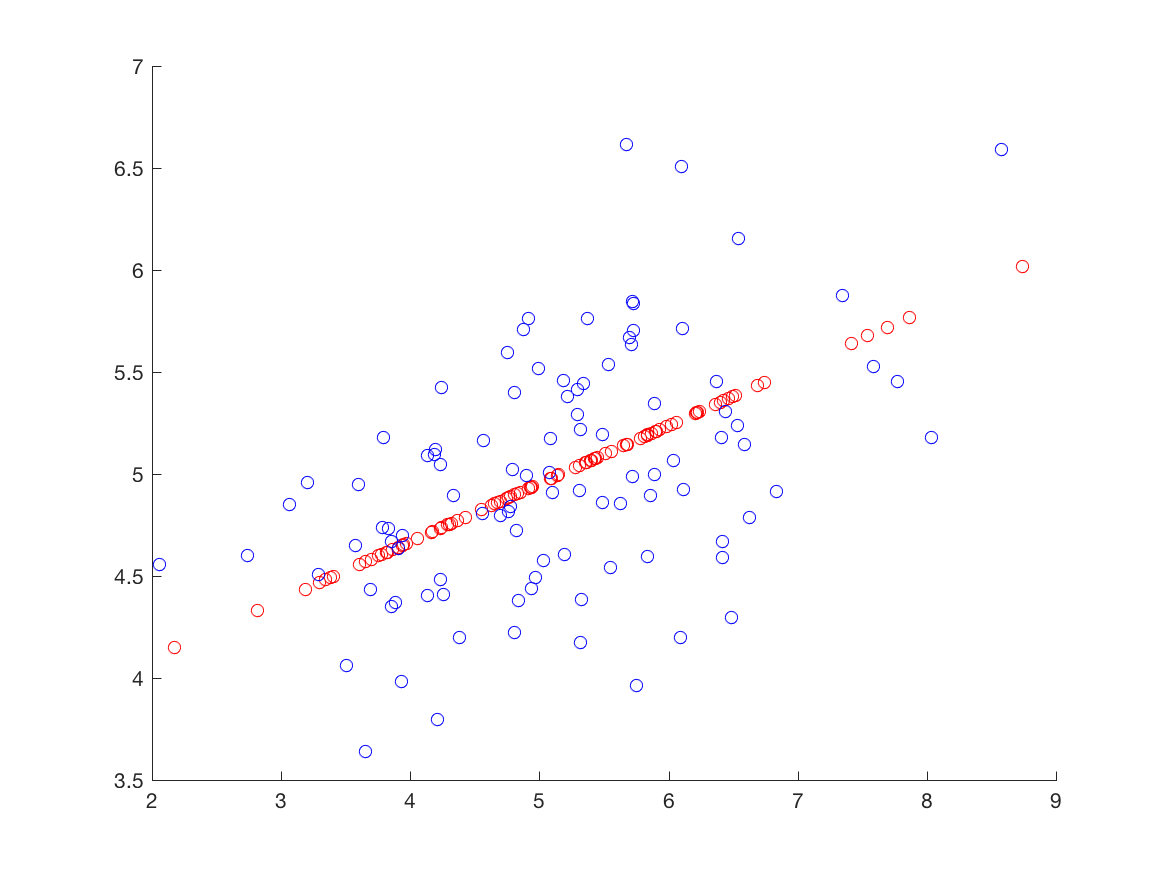
\includegraphics[width=0.93\textwidth]{../prolozeni-primkou.png}
    \end{center}

    \item Jaký je součet čtverců kolmých vzdáleností bodů k nalezené přímce?

    S využitím spektrálního rozkladu vstupní matice \( A \), nalezneme součet vzdáleností jako součet prvních \( k \) vlastních čísel matice \( A \). Námi proložený podprostor je dimenze 1, tedy součet vzdáleností je nejmenší vlastní číslo.
    
    Výsledek je \( 24.2419 \).

    \item Nalezněte požadovanou přímku ve dvou různých reprezentacích:
    \[ \left\{ \bf{y} \in \bbR^2 \| \bf{y}^T \bf{x} = \alpha \right\} = \left\{ \bf{y}_0 + t \bf{s} \| t \in \bbR \right\} \]

    Pro obecnou rovnici přímky \( \left\{ \bf{y} \in \bbR^2 \| \bf{y}^T \bf{x} = \alpha \right\} \) stačí vzít první vlastní vektor matice \( A \). Vlastní vektory jsou navzájem kolmé a mají jednotkovou velikost. První vlastní vektor tedy tvoří ortogonální doplněk k podprostoru, jehož bázi tvoří druhý vlastní vektor. Lze ho tedy použít jako normálový vektor přímky.

    K vypočtení parametru \( \alpha \) stačí vzít libovolný bod patřící do podprostoru (např. těžiště) a z rovnice \( \bf{y}^T \cdot \bf{x} = \alpha \) získáme \( \alpha \).

    Po provedení výpočtu získáme
    \[ \alpha = -3.3931 \]

    K vypočtení parametrické rovnice přímky nám stačí bod, který náleží přímce, a směrový vektor přímky. Jako bod můžeme použít těžiště a směrový vektor je stejný jako báze daného podprostoru, tedy \( \bf{y}_0 \) je těžiště a
    \[ \bf{s} = \left[ -0.9617, -0.2740 \right]. \] \( \bf{s} \) je vlastní vektor z matice \( V \), má tedy jednotkovou délku.
\end{enumerate}

\newpage

\section{Úkol 2: Komprese sekvence z motion capture}

\begin{enumerate}
    \item Minimalizujte kritérium
    \[ \sum_{i = 1}^m \lVert \tilde{\bf{a}}_i - \bf{a}_i \rVert^2 \]
    za podmínky, že body \( \tilde{\bf{a}}_1, \dots, \tilde{\bf{a}}_m \) leží v afinním podprostoru dimenze \( r \). Výsledkem bude matice \( \tilde{\bf{A}} \) s řádky \( \tilde{\bf{a}}^T_1, \dots, \tilde{\bf{a}}^T_m \). Proveďte pro sekvenci \uv{Chůze} a pro pět různých hodnot \( r \in \left\{ 1, 2, 5, 10, 15 \right\} \).

    \begin{center}
        \begin{tabular}{| l | c | c | c | c | c |}
            \hline
            r         & 1          & 2          & 5          & 10         & 15         \\ \hline
            kritérium & 4.6166e+08 & 1.6925e+08 & 1.0453e+07 & 1.1982e+06 & 2.5626e+05 \\ \hline
        \end{tabular}    
    \end{center}

    \item Výsledné body vyjádřete jako lineární kombinace \( \tilde{\bf{a}} = \tilde{\bf{V}} \bf{y} \) bázových vektorů. Pro \( r = 2 \) nakreslete sekvenci vektorů \( \bf{y}_1, \dots, \bf{y}_m \) jako trajektorii v rovině. To samé udělejte i ve třírozměrném prostoru, tedy pro \( r = 3 \). Proveďte pro sekvence \uv{Tanec Makarena} a \uv{Chůze}.

    \begin{center}
        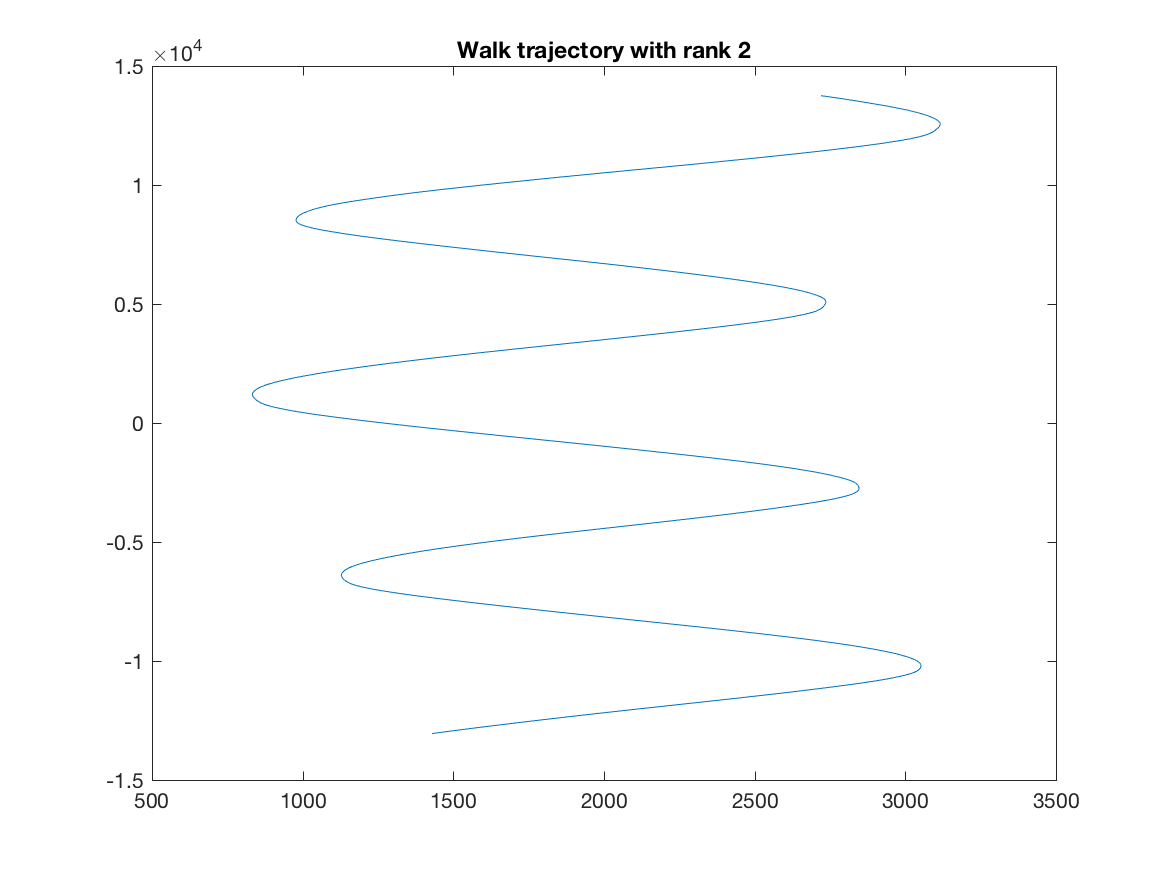
\includegraphics[width=0.8\textwidth]{../walk-r2.png}
        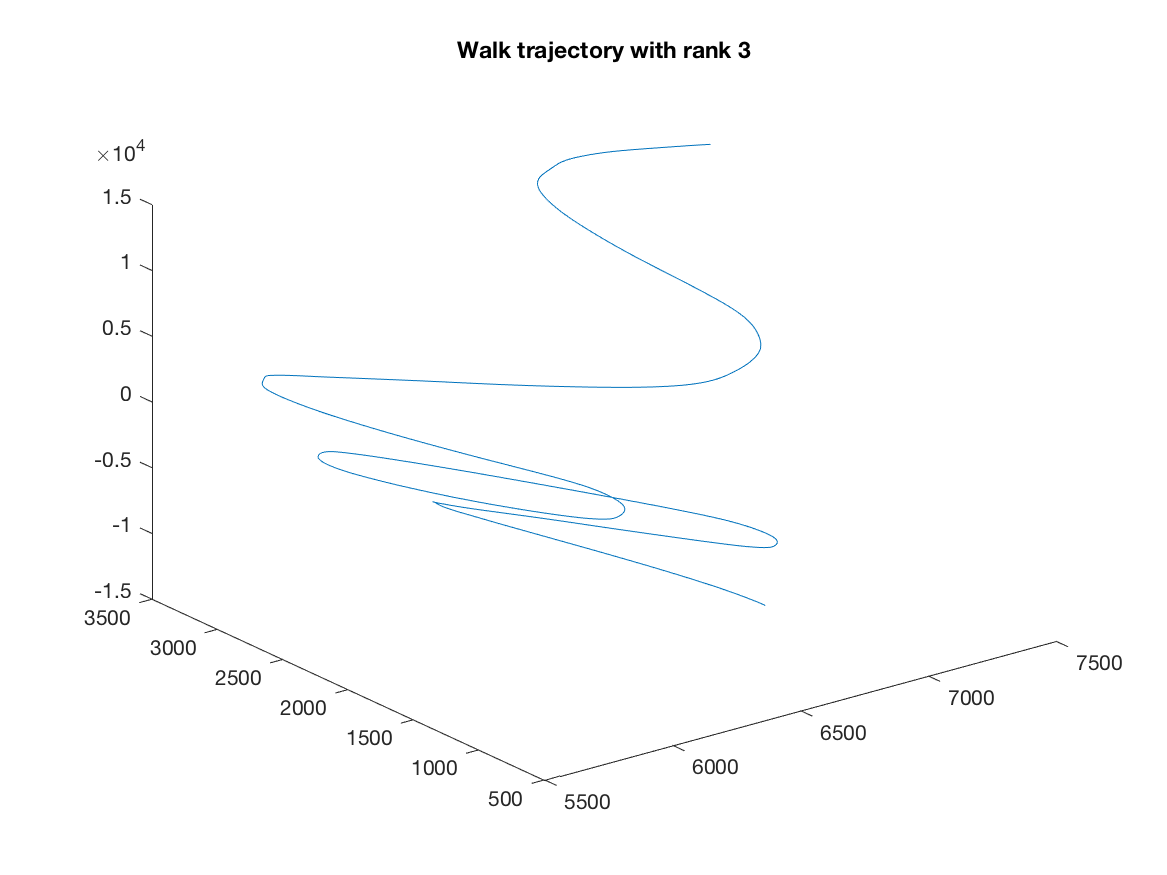
\includegraphics[width=0.8\textwidth]{../walk-r3.png}
        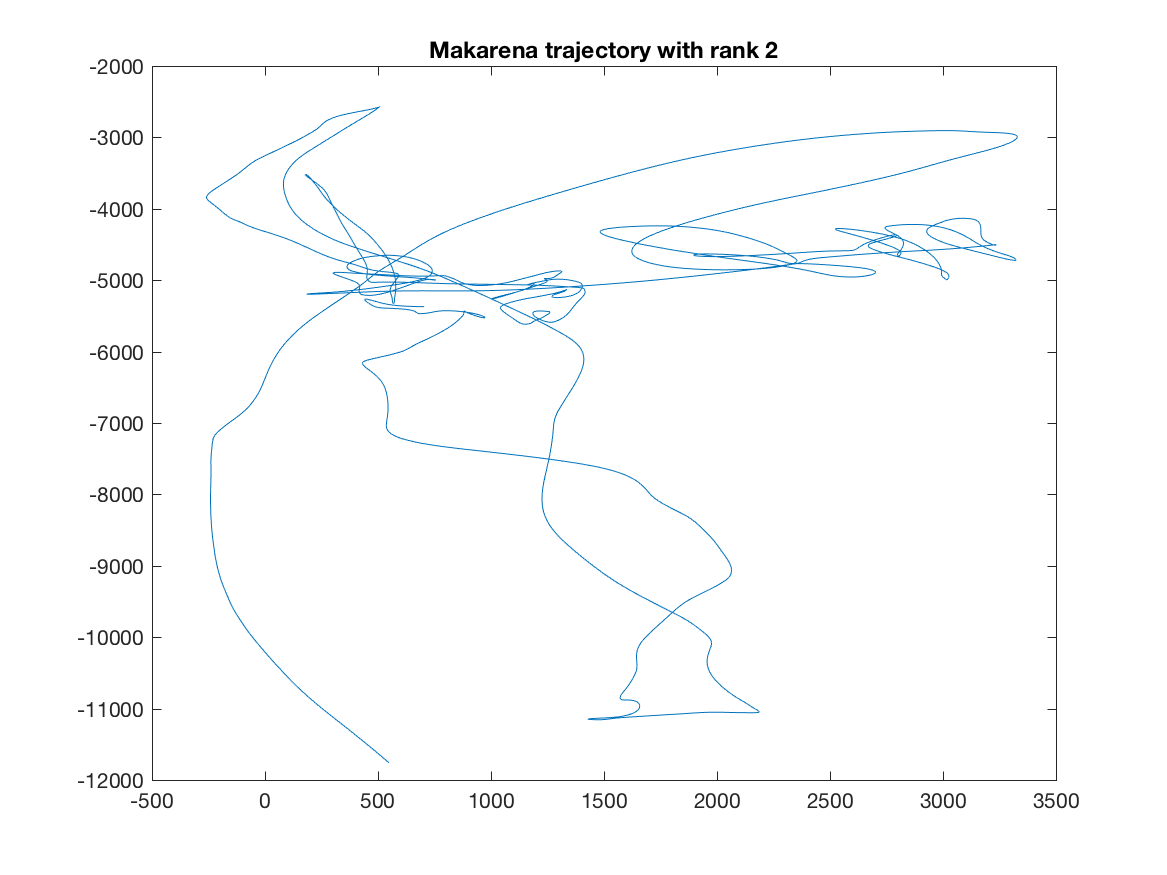
\includegraphics[width=0.8\textwidth]{../makarena-r2.png}
        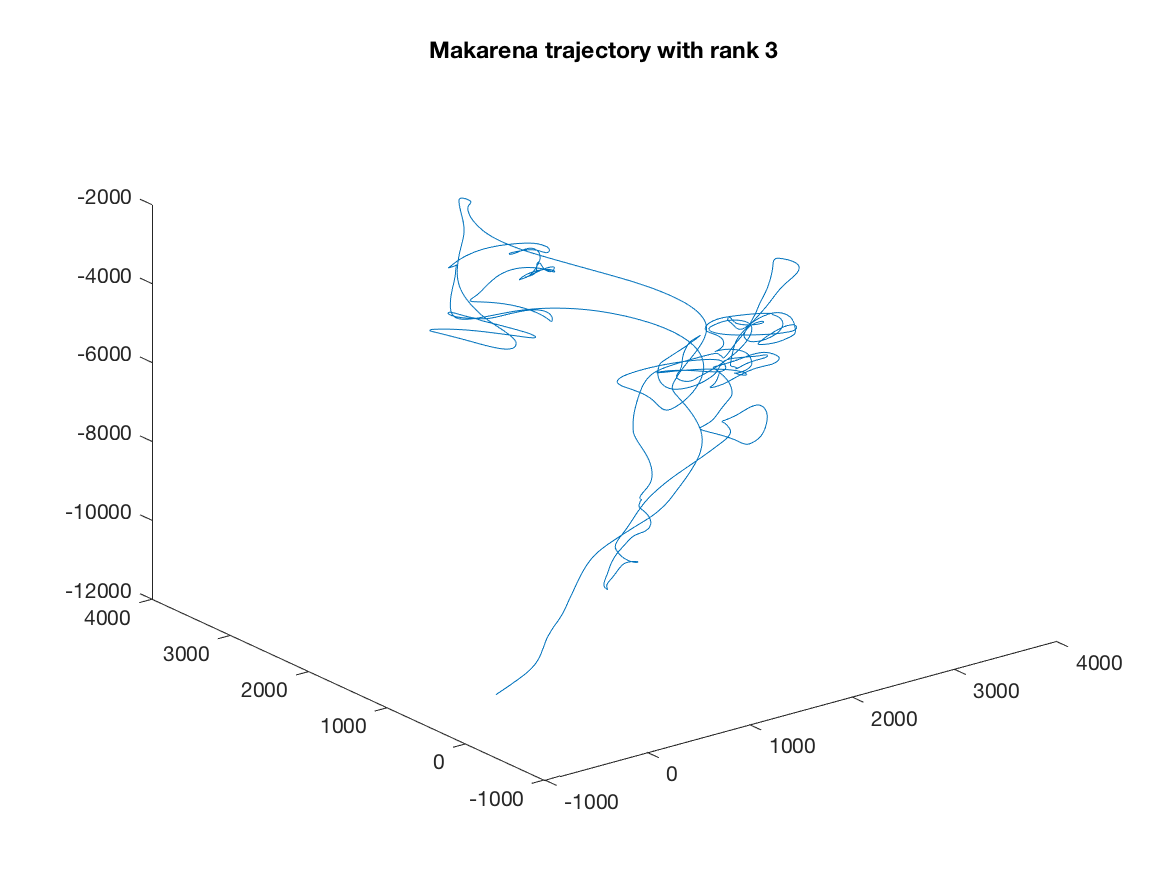
\includegraphics[width=0.8\textwidth]{../makarena-r3.png}
    \end{center}

    \item Uvažujte, že postava dělá čistý translační pohyb, tj. konfigurace bodů se nemění a jejich souřadnice se pohybují po přímce. Jaká je minimální dimenze podprostoru, aby aproximační chyba byla nulová?

    Jelikož se body pohybují po přímce, budou se měnit pouze jedna souřadnice a zbytek zůstane neměnný. Z toho výplývá, že dimenze podprostoru bude stejná jako dimenze přímky, tedy 1.
    
    \item Dejme tomu, že bychom chtěli spočítat optimální chybu aproximace
    \[ \sum_{i = 1}^m \lVert \tilde{\bf{a}}_i - \bf{a}_i \rVert^2 \]
    pro různé hodnoty \( r \leq n \). Dostali bychom tedy \( n \) čísel, z nichž poslední by bylo nulové. Jaký vztah mají tato čísla k singulárním číslům?

    Singulární čísla udávají nejmenší vzdálenost matice k jiné matici s nižší hodností. V našem případě se tedy singulární čísla rovnají optimální aproximační chybě.

\end{enumerate}

\newpage

\section{Příloha}

\subsection{Úkol 1}

\lstinputlisting[style=Matlab-editor]{../ukol_1.m}

\subsection{Úkol 2.1 - výpočet kritéria}

\lstinputlisting[style=Matlab-editor]{../ukol_2_2.m}

\subsection{Úkol 2.1 - aproximace vstupní matice}

\lstinputlisting[style=Matlab-editor]{../approximation.m}

\subsection{Úkol 2.2 - výpočet vektoru y}

\lstinputlisting[style=Matlab-editor]{../ukol_2_3.m}